\chapter{Experimentelle Untersuchungen}
\chaptermark{Experimentelle Untersuchungen}  % short form for headlines on pages
\label{ch:EntwickelteMethode}

\section{Angewendete Methodik}
\subsection{Testumgebung}

Um die Wirksamkeit der Parallelisierung der N++-Bibliothek in C++ zu bewerten, wird ein umfassender Benchmark-Test durchgeführt. Dieser Test umfasst verschiedene Kombinationen von Threads, Anzahl an Datensätzen und verschiedenen Computern mit verschiedenen Prozessorarchitekturen, um die Auswirkungen der Implementierung auf die Leistung der Bibliothek unter unterschiedlichen Bedingungen zu untersuchen.

Das C++ Programm wurde unter Einbindung der N++-Bibliothek auf dem jeweiligen System selbst kompiliert. Dabei wurde die Optimierungsstufe O2 verwendet, welche eine für Produktionssoftware gängige Optimierungsstufe ist. Die O2 Optimierungsstufe wendet fast jede Compileroptimierung an, die die Compiler zu bieten haben. Dabei werden lediglich als sehr unsicher eingestufte Optimierungen ausgelassen. Auf Linux wurde der GCC Compiler und auf MacOS der Clang Compiler verwendet, um native Binärdateien für die spezifische Prozessorarchitektur zu kompilieren. Das heißt, das Programm wurde nicht unter Emulation sondern vollständig nativ ausgeführt.

Die Tests wird mit unterschiedlichen Thread-Anzahlen ausgeführt, darunter 10, 8, 6, 4 und 2 gleichzeitig laufenden Threads, um den Einfluss der Parallelisierung auf die Ausführungsgeschwindigkeit zu untersuchen. Zusätzlich wird das Programm auch mit einem einzelnen Thread ausgeführt, um einen Vergleich mit der vorausgegangenen Implementierung herstellen zu können. Für jede Thread-Anzahl werden außerdem verschiedene Größen an Datensätzen getestet. Die Größe der Datensätze wird über die Anzahl an Partitionen spezifiziert. Eine Partition bedeutet dabei, dass die gesamte Datenmenge verwendet wird, wohingegen 4 Partitionen bedeuten, dass nur ein Viertel, also 25\% der Datenmenge verwendet werden. Das Programm wird in diesem Test mit 1, 2, 4 und 8 Partitionen getestet, wobei es auf dem langsamsten Computer nur auf 4 und 8 beschränkt wurde.

Für jede Kombination von Threads und Partitionen werden mindestens 5 Testläufe durchgeführt, um robuste Durchschnittswerte zu erhalten und Schwankungen zu minimieren. Gemessen wird die benötigte Zeit für den gesamten Programmdurchlauf in Sekunden. Vor jedem Durchlauf werden die Testgeräte auf einen neutralen Zustand zurückgesetzt, um faire Vergleichsbedingungen sicherzustellen. Dies wird gewährleistet, indem gleiche Seeds für die Zufallszahlgeneratoren verwendet werden, und sichergestellt wird, dass keine anderen Programme laufen.
Das Ergebnis jedes Programmdurchlaufs wird in eine Datei geschrieben, um vergleichen zu können, ob mit verschiedenen Anzahlen von Threads die gleichen Ergebnisse berechnet werden.

Nach Abschluss der Testläufe werden die erzielten Ergebnisse automatisch analysiert und Durchschnittswerte für jede Kombination von Threads und Partitionen berechnet. Diese Durchschnittswerte dienen dazu, die möglichen Schwankungen der Testabläufe auszugleichen, und ein neutraleres Ergebnis zu liefern.

\subsection{Benchmark Script}

Aus 6 verschiedenen Anzahlen an Threads, 4 verschiedenen Größen der Datensätze und 5 Durchläufen pro Kombination ergeben sich 120 einzelne Tests, die pro System ausgeführt werden müssen.
Um diese Arbeit zu erleichtern und einen reproduzierbaren Testprozess zu ermöglichen habe ich ein Skript geschrieben, welches alle Tests nacheinander automatisch ausführt.

Das Skript misst die benötigten Laufzeiten der Durchläufe und schreibt nach jedem Durchlauf die benötigte Zeit in eine Datei. Zusätzlich werden die Zeit und Informationen zu jedem Durchlauf auch in eine CSV Datei geschrieben, um das Auswerten der Benchmarks auf einem System durch nur eine einzige Datei zu ermöglichen.

Als Parameter ist es möglich, die maximale Anzahl an Threads festzulegen. So ist es beispielsweise auf einem Raspberry Pi sinnvoll, das Programm nur mit maximal 4 Threads zu testen, da er nur über 4 Threads verfügt.

Das Skript ist simpel und wurde in Bash geschrieben, was die Portabilität zwischen Linux und MacOS gewährleistet. Dabei wurde jedoch das Programm bc verwendet, welches auf Linux standardmäßig nicht vorinstalliert ist.

\begin{figure}[H]
\begin{minted}
[
frame=lines,
framesep=2mm,
baselinestretch=1.2,
fontsize=\footnotesize,
linenos
]{bash}
#!/bin/bash
ATTEMPTS=5
PARTITIONS=(8 4 2 1) # Verschiedene Partitionen zum Testen
THREADS=(10 8 6 4 2 1) # Verschiedene Thread Anzahlen zum Testen
AVAILABLE_THREADS=10 # Maximal verfügbare Anzahl an Threads für aktuelles System

function run_attempt {
    # Hier wird ein Durchlauf durchgeführt und getestet
}

# Test für jede mögliche Kombination durchführen
for partition in ${PARTITIONS[@]};do
  for threads in ${THREADS[@]};do
      if ((threads <= AVAILABLE_THREADS));then
        for ((i = 1; i <= ATTEMPTS; i++)); do
          run_attempt "$threads" "$partition" "$i"
        done
      fi
    done
done
\end{minted}
\caption{Vereinfacht dargestelltes Benchmark Skript}
\label{fig:benchmark_script_code}
\end{figure}

\section{Ergebnisse}

\subsection{Apple M1 Pro}

Der M1 Pro Prozessor, der im MacBook Pro 16 Zoll verwendet wird, integriert eine heterogene Mehrkernarchitektur, die auf die Parallelverarbeitung von Aufgaben ausgelegt ist. Der M1 Pro wurde 2021 vorgestellt und ist eine hochskalierte Version des M1 Prozessors. Er verfügt über insgesamt 12 CPU-Kerne, darunter 8 Hochleistungskerne und 4 Effizienzkerne \citep{MacBook_Technische_Daten}. Die Hochleistungskerne sind für rechenintensive Aufgaben konzipiert, während die Effizienzkerne für weniger anspruchsvolle Aufgaben und eine Reduzierung des Energieverbrauchs optimiert sind.

In Bezug auf die Leistung bietet der M1 Pro Prozessor eine sehr beeindruckende Single-Core-Leistung sowie eine bemerkenswerte parallele Verarbeitungsfähigkeit für multithreaded Anwendungen. Die genaue Hauptspeichergröße beträgt 16 GB RAM mit einer Speicherbandbreite von 200 GBit/s \citep{MacBook_Technische_Daten}. Auch die Cache-Größe des Prozessors ist sehr hoch, was die Latenz bei Speicherzugriffen zusätzlich vermindert.

\begin{figure}[H]
\centering
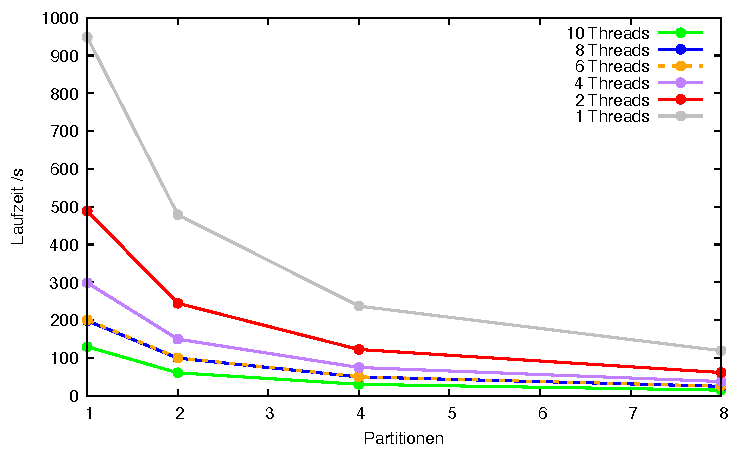
\includegraphics[width=0.8\textwidth]{../results/plots/m1pro/comp_all_threads.pdf}
\caption{Ergebnisse der Leistungstests verglichen nach Thread Anzahl}
\label{fig:m1pro_benchmark_threads}
\end{figure}

\begin{figure}[htbp!]
\centering
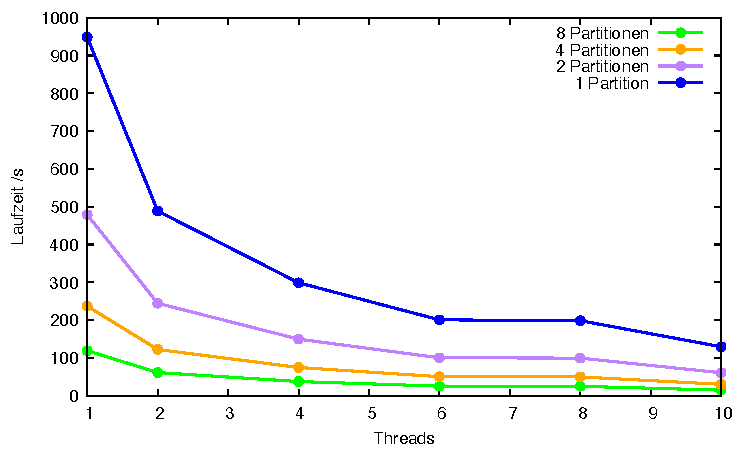
\includegraphics[width=0.8\textwidth]{../results/plots/m1pro/comp_all_partitions.pdf}
\caption{Ergebnisse der Leistungstests verglichen nach Datensatzgröße}
\label{fig:m1pro_benchmark_partitions}
\end{figure}

\subsection{AMD Ryzen 3600XT}
Der AMD Ryzen 5 3600XT ist ein Prozessor aus der Ryzen 3000-Serie von AMD, der im Jahr 2020 eingeführt wurde. Er verfügt über insgesamt 6 CPU-Kerne und 12 Threads auf Basis der Zen 2-Architektur, welche auch im Servermarkt verbreitet ist. Es handelt sich um einen Desktopprozessor mit einer maximalen Leistungsaufnahme von 95 Watt \citep{Ryzen_Technische_Daten}.

Der Prozessor unterstützt DDR4-RAM mit unübertakteten Geschwindigkeiten von bis zu 3200 MHz \citep{Ryzen_Technische_Daten}. Die genaue Speicherbandbreite und Größe hängt von der verwendeten RAM-Konfiguration ab, da Desktop Prozessoren modular in verschiedene Systeme eingebaut werden können.

In Bezug auf den Cache verfügt der Ryzen 5 3600XT über 32KB L1-Cache, 512KB L2-Cache und 32MB L3-Cache pro Kern  \citep{Ryzen_Technische_Daten}. In der Konfiguration des Testcomputers sind 16GB DDR4 Speicher mit 3600 MHz verbaut, und der Prozessor wird mit einer Wasserkühlung gekühlt, was für eine gleichmäßige und Robuste Kühlung sorgt.

\begin{figure}[htbp!]
\centering
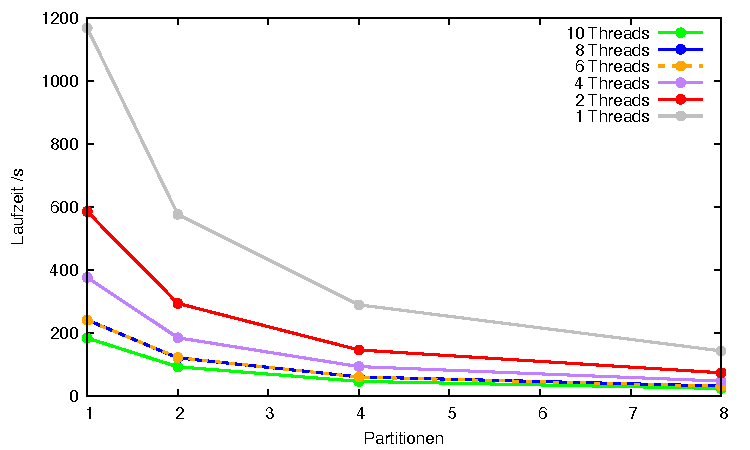
\includegraphics[width=0.8\textwidth]{../results/plots/3600xt/comp_all_threads.pdf}
\caption{Ergebnisse der Leistungstests verglichen nach Thread Anzahl}
\label{fig:ryzen_benchmark_threads}
\end{figure}

\begin{figure}[htbp!]
\centering
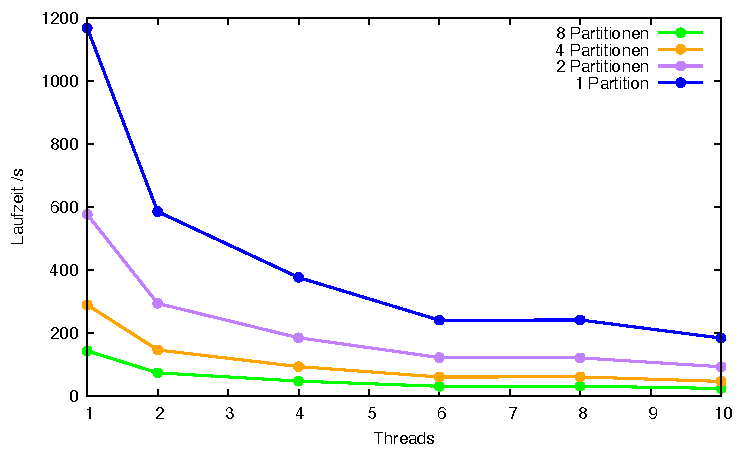
\includegraphics[width=0.8\textwidth]{../results/plots/3600xt/comp_all_partitions.pdf}
\caption{Ergebnisse der Leistungstests verglichen nach Datensatzgröße}
\label{fig:ryzen_benchmark_partitions}
\end{figure}

\subsection{Raspberry Pi 3}
Der Raspberry Pi 3 ist ein Single-Board-Computer, der von der Raspberry Pi Foundation entwickelt wurde. Ein Single-Board-Computer ist eine vollständige Computerplatine, die alle erforderlichen Komponenten wie Prozessor, Speicher, Ein-/Ausgabeanschlüsse und Stromversorgung auf einer einzigen Platine vereint. Der Raspberry Pi 3 wurde 2016 veröffentlicht und basiert auf einem ARM Cortex-A53 Quad-Core-Prozessor mit einer Taktfrequenz von 1,2 GHz und 1 GB LPDDR2-RAM \citep{RaspberryPi_Technische_Daten}.

Im Vergleich zu anderen Prozessoren ist der Raspberry Pi 3 natürlich langsamer. Seine Spezifikationen bieten eine grundlegende Leistung für einfache Computing-Aufgaben und den Betrieb von IoT (Internet der Dinge)-Anwendungen.

Der Raspberry Pi 3 ist aufgrund seiner geringen Größe, seines geringen Stromverbrauchs und seiner vielfältigen Einsatzmöglichkeiten beliebt. Er wird häufig in Bildungsprojekten, DIY (Do It Yourself)-Projekten, Heimautomatisierungssystemen und als kostengünstige Entwicklungsumgebung für Softwareentwickler eingesetzt. Trotz seiner begrenzten Leistungsfähigkeit erfüllt der Raspberry Pi 3 wichtige Funktionen in verschiedenen Anwendungsbereichen aufgrund seiner Kompaktheit und seines erschwinglichen Preises.

Aufgrund der begrenzten Leistung des Raspberry Pi 3 und der damit verbundenen Laufzeiten konnte der Testablauf nicht vollständig durchgeführt werden. Es wurden maximal 4 Threads getestet, und die Partitionen wurden auf 8 und 4 begrenzt.

\begin{figure}[H]
\centering
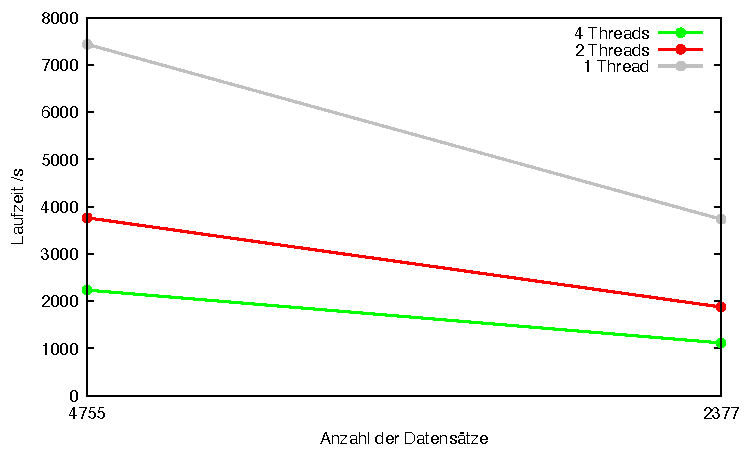
\includegraphics[width=0.8\textwidth]{../results/plots/raspberrypi3/comp_all_threads.pdf}
\caption{Ergebnisse der Leistungstests verglichen nach Thread Anzahl}
\label{fig:raspi_benchmark_threads}
\end{figure}

\begin{figure}[htbp!]
\centering
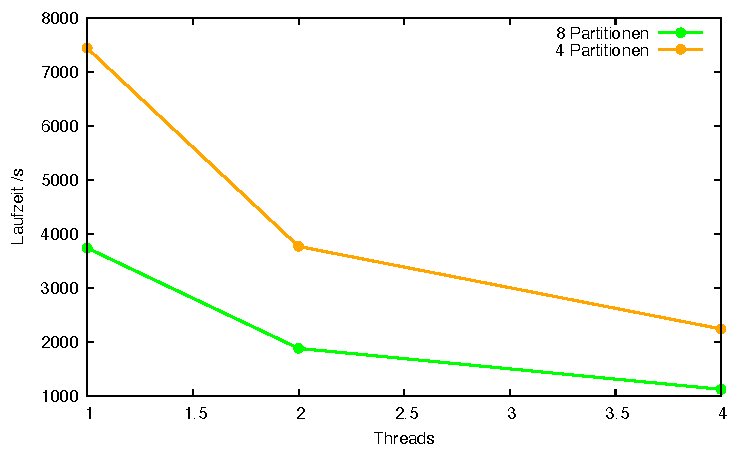
\includegraphics[width=0.8\textwidth]{../results/plots/raspberrypi3/comp_all_partitions.pdf}
\caption{Ergebnisse der Leistungstests verglichen nach Datensatzgröße}
\label{fig:raspi_benchmark_partitions}
\end{figure}

\subsection{Cloud Server}

\section{Auswertung}

\newpage
